\chapter{Multi-Layer Perceptrons}
\label{ch:lesson32}

Chapter~\ref{ch:lesson31}'s single neuron, trained however carefully, could not beat chance on the ring-inside-a-disk dataset --- a single linear projection just isn't expressive enough (Figure~\ref{fig:l32-1}). This chapter adds one more layer: instead of \emph{one} projection followed by a threshold, use \emph{two} projections with a nonlinearity in between. That's it. That's the entire idea behind every deep network in this course --- stack more of these.

\begin{figure}[h]
\centering
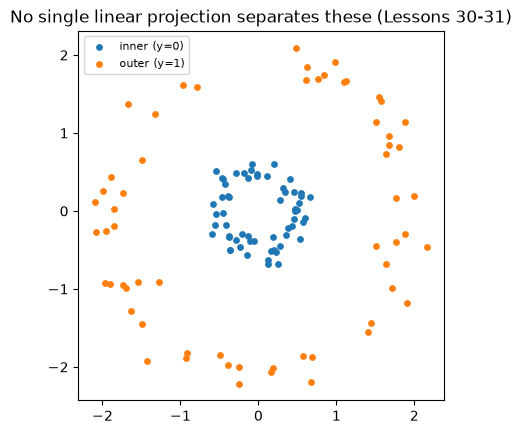
\includegraphics[width=0.55\textwidth]{figures/lesson32_fig01.png}
\caption{The ring-and-disk dataset --- no single linear projection separates these (Chapters~\ref{ch:lesson30}--\ref{ch:lesson31}).}
\label{fig:l32-1}
\end{figure}

\section{Two projections, one nonlinearity}

A \textbf{multi-layer perceptron (MLP)} chains a \emph{hidden} projection into a new space, a nonlinear \textbf{activation} applied elementwise, and then a final linear projection (exactly Chapter~\ref{ch:lesson31}'s neuron) on top of the \emph{transformed} coordinates:
\begin{equation}
h = \text{ReLU}(W_1x+b_1), \qquad z=w_2^\top h+b_2, \qquad p=\sigma(z).
\end{equation}
$\text{ReLU}(u)=\max(0,u)$ is the simplest common activation: linear everywhere except a single kink at zero. That one kink, applied independently to every unit of $h$, is enough --- the hidden layer can bend, fold, and stretch the input space so a \emph{linear} boundary in the transformed space corresponds to a highly nonlinear boundary back in the original coordinates.

\subsection*{Why the nonlinearity is essential}

Without ReLU --- if the hidden layer were left as plain $h=W_1x+b_1$ --- the two layers would collapse into a single linear projection:
\begin{equation}
z = w_2^\top(W_1x+b_1)+b_2 = \underbrace{(w_2^\top W_1)}_{w'^\top}x + \underbrace{(w_2^\top b_1+b_2)}_{b'}.
\end{equation}
That's exactly Chapter~\ref{ch:lesson31}'s single neuron again, just with the two layers' weights multiplied together into one $w'$ and $b'$. This is the flip side of Chapter~\ref{ch:lesson30}'s observation that matrix multiplication is projection, stacked: composing two matrix multiplications is \emph{still} just one matrix multiplication, so stacking purely linear layers buys nothing, no matter how many are chained. ReLU's kink is what breaks that collapse --- because it isn't a linear function, $w_2^\top\text{ReLU}(W_1x+b_1)+b_2$ can no longer be rewritten as any single $w'^\top x+b'$. Verified directly: passing the same random data through two \emph{linear} layers matches the single combined layer $W_1W_2$, $b_1W_2+b_2$ to within $1.78\times10^{-15}$.

\section{Backprop through two layers}

The chain rule extends cleanly: propagate the error signal $\partial L/\partial z$ from Chapter~\ref{ch:lesson31} backward through the output projection to get $\partial L/\partial h$, then backward through the ReLU and the hidden projection to get $\partial L/\partial W_1,\partial L/\partial b_1$. Every step is either ``multiply by a weight matrix's transpose'' or ``multiply elementwise by an activation's derivative'' --- this is \emph{all} backpropagation ever is, no matter how many layers are stacked. A from-scratch implementation of forward and backward passes through a 2-layer MLP matches PyTorch's autograd gradients to within $3\times10^{-17}$ on every parameter.

\section{Training}

\begin{lstlisting}
def forward(X, W1, b1, W2, b2):
    a1 = relu(X @ W1 + b1)
    z2 = (a1 @ W2 + b2).ravel()
    return sigmoid(z2), (X, a1)
\end{lstlisting}

With $H=4$ hidden units, trained for 3000 epochs: final accuracy $100.0\%$ (Chapter~\ref{ch:lesson31}'s single neuron managed only $50\%$ on this dataset), shown in Figure~\ref{fig:l32-2}.

\begin{figure}[h]
\centering
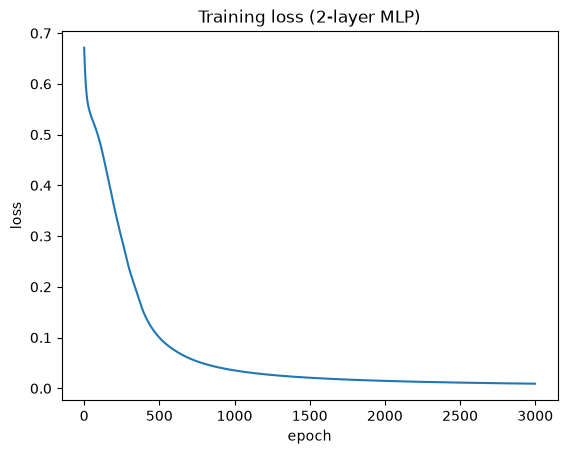
\includegraphics[width=0.5\textwidth]{figures/lesson32_fig02.png}
\caption{Training loss (2-layer MLP) over 3000 epochs.}
\label{fig:l32-2}
\end{figure}

\section{The hidden layer's projections, made visible}

Each hidden unit is itself a Chapter~\ref{ch:lesson30}-style projection: a direction $w_i$ (one column of $W_1$) and an offset $b_i$ (one entry of $b_1$), together defining a cut $w_i\cdot x+b_i=0$ that ReLU zeroes out on one side of. With only 2 input dimensions, all $H$ of these can be drawn directly over the original data, as Figure~\ref{fig:l32-3} shows.

\begin{figure}[h]
\centering
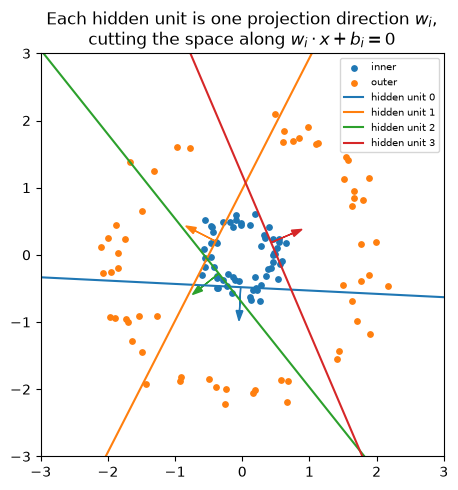
\includegraphics[width=0.5\textwidth]{figures/lesson32_fig03.png}
\caption{Each hidden unit is one projection direction $w_i$, cutting the space along $w_i\cdot x+b_i=0$.}
\label{fig:l32-3}
\end{figure}

On its own, each cut is just a straight line --- no single one of them separates the ring from the disk. But the output layer combines all $H$ of their (ReLU'd) results together, and a handful of straight cuts arranged around the ring, combined with the right weights, can approximate a closed curve well enough to enclose it.

\subsection*{What the hidden layer actually did}

The output layer is \emph{just} a linear projection (Chapter~\ref{ch:lesson31}'s neuron) --- but it acts on $h$, the hidden layer's output, not on the original $x$. If the hidden layer did its job, the \emph{transformed} points should already be much easier to separate with a straight line. Since $h$ lives in $\mathbb{R}^4$ here, PCA (Chapter~\ref{ch:lesson06}) visualizes it in 2D, shown alongside the original space in Figure~\ref{fig:l32-4}.

\begin{figure}[h]
\centering
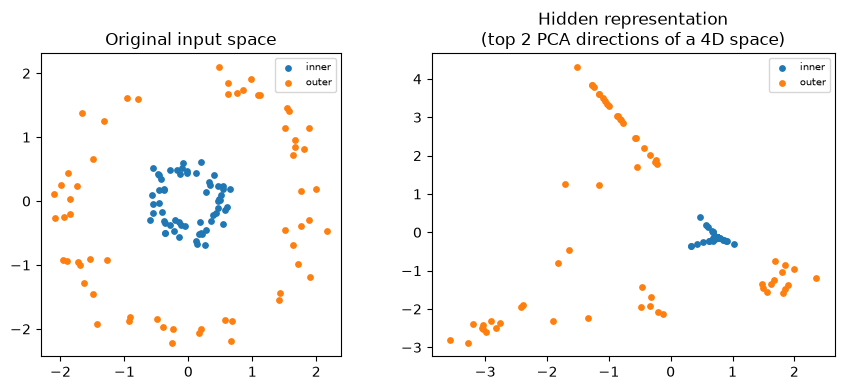
\includegraphics[width=0.9\textwidth]{figures/lesson32_fig04.png}
\caption{Original input space vs.\ the hidden representation (top 2 PCA directions of a 4D space).}
\label{fig:l32-4}
\end{figure}

Even this lossy 2D snapshot of the full 4D hidden space shows the two classes pulled apart into something close to linearly separable --- a big improvement over the $74\%$ ceiling that was the best \emph{any} line could do in the original space (Chapter~\ref{ch:lesson30}). The actual output neuron works in the full 4D hidden space, where it achieves 100\% accuracy exactly. This is the entire mechanism of deep learning in miniature: each layer \emph{reshapes the space} so that the next layer's job gets easier, until the final layer's job is trivial --- a single linear projection.

\section{Model capacity: how many hidden units are enough?}

A model's \textbf{capacity} is how rich a family of functions it can represent. Here that's set directly by $H$, the hidden layer's width: each hidden unit contributes one straight cut, and the output layer combines these units. Too few units, and the model simply cannot represent the boundary needed by the dataset --- no amount of training can find a solution that doesn't exist. Sweeping $H$ and retraining from scratch at each width, across 5 random initializations each:

\begin{center}
\renewcommand{\arraystretch}{1.3}
\begin{tabular}{rrrr}
\hline
\textbf{$H$} & \textbf{mean acc} & \textbf{min} & \textbf{max} \\
\hline
1  & 72.0\%  & 70.8\% & 73.3\% \\
2  & 89.5\%  & 67.5\% & 95.8\% \\
3  & 89.5\%  & 72.5\% & 100.0\% \\
4  & 100.0\% & 100.0\% & 100.0\% \\
6  & 100.0\% & 100.0\% & 100.0\% \\
8  & 100.0\% & 100.0\% & 100.0\% \\
16 & 100.0\% & 100.0\% & 100.0\% \\
\hline
\end{tabular}
\end{center}

\begin{figure}[h]
\centering
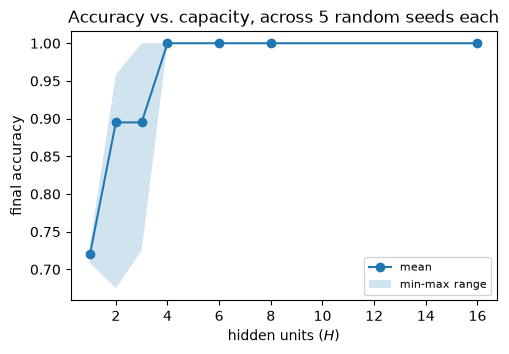
\includegraphics[width=0.55\textwidth]{figures/lesson32_fig05.png}
\caption{Accuracy vs.\ capacity, across 5 random seeds at each width.}
\label{fig:l32-5}
\end{figure}

$H=1$ (Figure~\ref{fig:l32-5}) caps out well below 100\% no matter how long it trains or which seed it starts from --- that's not an optimization failure, it's a representational ceiling: one hidden unit is just a single cut, so it inherits Chapter~\ref{ch:lesson30}'s $\sim74\%$ linear limit almost exactly. $H=2$ is better, but still capacity-limited --- none of the five seeds reach 100\%. $H=3$ is the actual knife's edge: the capacity to represent a perfect solution is there (one seed reaches exactly 100\%), but whether training finds it depends on \emph{which} seed it starts from (a preview of Chapter~\ref{ch:lesson33}'s optimization landscape problems).

By $H=4$, every seed reaches 100\% reliably: there's enough capacity that the network stops being the bottleneck, and training reliably finds a solution within that capacity. This is the general shape of a capacity curve --- a hard floor set by what the model \emph{can} represent, with optimization difficulty riding on top of it near the floor's edge. This same curve is revisited in Chapter~\ref{ch:lesson35} from the opposite direction: there, capacity is held generously high and \emph{data} is scarce, which turns ``enough capacity to represent the right answer'' into ``also enough capacity to memorize the wrong one.''

Width isn't the only knob. \textbf{Depth} --- stacking more layers instead of making a layer wider --- is the other axis, and it isn't just ``width in disguise'': a deep, narrow network can represent some functions far more compactly than a shallow, wide one needs to, but it introduces its own failure mode instead. Chapter~\ref{ch:lesson37} picks this up directly: stacking enough layers can make gradients vanish before they ever reach the earliest ones, a problem not encountered by this chapter's shallow 2-layer network.

\subsection*{Exercises}
\begin{enumerate}
  \item The capacity sweep above used ReLU. Rerun it with \code{tanh} instead. Does the same $H=1$ ceiling and $H=3$-to-$H=4$ transition appear, or does a smooth activation change where the floor sits?
  \item Replace \code{relu}/\code{relu\_deriv} with \code{tanh}/its derivative ($1-\tanh^2$) throughout, and retrain. Does it still solve the problem? Compare the resulting loss curve's shape to the ReLU version's.
  \item Remove the nonlinearity entirely (replace \code{relu(z1)} with just \code{z1}). Confirm the network can no longer beat Chapter~\ref{ch:lesson31}'s $\sim50\%$ ceiling --- consistent with the collapse-to-a-single-projection argument above, now demonstrated on actual training dynamics instead of just static algebra.
\end{enumerate}

\vfill
\fullcode{lesson32}{lesson32_multilayer_perceptrons}
